\section{Theoretische Grundlagen} 
\subsection{Terraform}
\begin{otherlanguage}{ngerman}
\subsubsection{Funktionsweise}
\textit{Terraform} ist eine \textit{Open-Source-Software}, welche die Vorbereitung von \textit{Cloud Servern} einfacher macht. Sie wurde von HashiCorp dazu entwickelt, Infrastrukturen vorzubereiten und zu verwalten.\footcite{introform} Mit Infrastrukturen sind hier \textit{virtuelle Maschinen} verschiedenster Anbieter gemeint.\footnote{\cite{Terraform}} Terraform hat lizenzierte Provider für die seine Dienste anwendbar sind.\footcite{TerraProviders} Durch die hohe Konnektivität dieser Software sind die Einsatzorte sehr vielseitig. Das macht die Software in der Entwicklung und im Betrieb von Unternehmen sehr attraktiv. 
\newline
\newline
Terraform ist ein Infrastructure-as-Code-Tool und wird für die Bereitstellung von physischen als auch virtuellen Servern verwendet. Das Tool arbeitet mit Konfigurationsdateien, die in der HashiCorp Configuration Language(HCL) geschrieben werden. Die genannten Dateien sind von Menschen lesbar. Zudem ist HCL eine deklarative Sprache. Das heißt, dass der Nutzer den Wunschaufbau der Cloud-Umgebung in der Terraform-Datei beschreibt. Die einzelnen Schritte um den gewünschten Zustand zu erreichen, werden von Terraform übernommen. 
\newline
Die Prozesse in die die Arbeit mit Terraform unterschieden werden kann, sind in drei Schritte aufgeteilt. Der erste Schritt ist \tt write \rm. In dieser Phase wird der Code definiert. Dafür werden die benötigten Ressourcen für die jeweiligen Provider definiert und Terraform-Konfigurations-Dateien mit der Endung \tt .tf \rm verwendet. Aus diesen Dateien entnimmt Terraform beispielsweise welcher Cloud-Anbieter verwendet wird. Als Beispiel für einen Anbieter mit dem Terraform funktioniert kann die \dq Hetzner-Cloud \dq{} genannt werden. Zu den Providern findet sich auf der Seite von Terraform eine jeweilige Dokumentation darüber, wie die Ressourcen einzubinden sind. Der Code der Konfigurations-Dateien entscheidet darüber, wie die virtuelle Umgebung konfiguriert wird, wenn das Skript ausgeführt wird. 
\newpage
\tt  
\begin{lstlisting}[caption = Block in HCL - Syntax, language=python, numbers=left, numberstyle=\tiny]
  #Create a server
  resource "hcloud_server" "malware" {
    name        = "forensics"
    image       = "ubuntu-22.04"
    server_type = "cx11"
    firewall_ids = [hcloud_firewall.saferfw.id]
    ssh_keys = [hcloud_ssh_key.default.id]
    user_data = file("user_data.yml")
  }
\end{lstlisting}
\rm
\newline
\newline
Im obigen Code ist der allgemeine Aufbau eines Blocks in Terraform zu erkennen. Ein Block beginnt mit dem \tt type \rm . Er legt auch fest, welche und wie viele sogennante Bezeichner folgen müssen. Dieser Typ ist hier in Zeile zwei als \dq resource \dq{} festgelegt. Als Bezeichner folgen \dq hcloud\_server \dq{} und \dq malware\dq{}. Wir definieren hier also einen Server in der Hetzner-Cloud mit dem Namen \dq malware\dq{}. Der Inhalt des Blocks befindet sich in geschweiften Klammern. In diesen Klammern sind zusätzliche Argumente zu finden. Diese bestimmen die Abhängigkeiten und die Zusammenhänge mit anderen Blocks und Argumenten. Die Abhängigkeiten von anderen Netzwerkkomponenten sind in Zeile sechs zu erkennen. Hier wird die Firewall dem Server zugewiesen. Auch der SSH-Key ist in Zeile acht festgelegt.
\newline
Wenn der Code verfasst wurde, folgt der nächste Schritt im Arbeitsablauf von Terraform. Hier sollten die Konfigurationsdateien, die verfasst wurden, initialisiert werden. Dies geschieht mit dem Befehl \tt terraform init \tt. Anschließend kann für das weitere Vorgehen ein plan erstellt werden. Durch \tt terraform apply \rm wird dieser Plan erstellt und ausgegeben. Um Fortzufahren muss der Plan, indem jeder Schritt aufgelistet ist, den Terraform durchführen wird, bestätigt werden. Diese einzelnen Schritte können Änderungen, Löschungen oder das Hinzufügen von Dateien sein.
\newline
\begin{figure}[h]
    \centering
    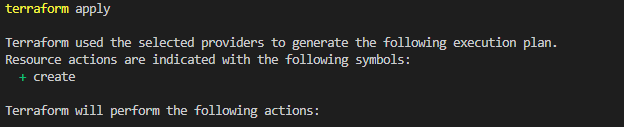
\includegraphics{LaTeX/graphic/terraformapply.png}
    \caption{Terraform - Planungsphase}
\end{figure}
%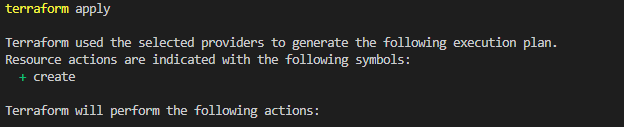
\includegraphics[]{LaTeX/graphic/terraformapply.png}
\newline 
 
Die Dritte und letzte Phase im Terraform-\it Workflow \rm ist \tt terraform apply\rm. Sie beginnt mit der Bestätigung des Plans. Ab diesem Zeitpunkt beginnt Terraform mit der Bereitstellung der Cloud-Umgebung. Woraus diese besteht, ist von den Konfigurationsdateien abhängig. 

\subsubsection{Vorteile}
Terraform birgt einige nützliche Vorteile. Einer dieser ist die Flexibilität. Durch die Vielzahl an Providern kann diese gewährleistet werden. Diese Provider lassen das Provisioning einer Cloud-Umgebung mittels Terraform zu. So kann beispielsweise eine Konfiguration für einen Hetzner-Server mit wenigen Änderungen verwendet werden, um eine virtuelle Umgebung bei \dq Oracle \dq{} zu erstellen. Diese Flexibilität ist besonders für dieses Projekt interessant, denn so kann die virtuelle Umgebung bei verschiedenen Anbietern konfiguriert und verwendet werden. 
\newline 
Ein weiterer Vorteil, der sich daraus ergibt, ist, dass Terraform an sich sehr schnell ist. Mit den Befehlen \tt init\rm und \tt apply\rm wird eine virtuelle Umgebung mit den gewünschten Konfigurationen erstellt. Das ist gegenüber dem manuellen Einrichten einer virtuellen Umgebung sehr zeitsparend. 
\newline
Hinzu kommt, dass Terraform gut zu verstehen ist. Die Sprache in der die Konfigurationsdateien geschrieben ist, ist sehr intuitiv und gut verständlich. Wenn die Syntax einmal begriffen wurde, lässt sich aus den Konfigurationsdateien gut auf das Endprodukt schließen. Natürlich sind virtuelle Umgebungen, die von Grund auf komplex sind, auch in Terraform komplex. Dennoch ist die Verständlichkeit der Sprache eine positive Anmerkung wert.
\newline
Weiterhin ist für IT-Teams die Planungsphase ein gutes Tool, um Veränderungen bereits im Vorweg zu sehen und Folgen abschätzen zu können. Dabei können Fehler, die zu einem unerwünschten Ergebnis führen, frühzeitig erkannt und vermieden werden.
\end{otherlanguage}